% Extensión estimada: unas 3 páginas, una subsección, dos tablas y una figura (ficha 4.4).
% Fuentes: ficha fichas/04-resultados-clasificacion/04-comparacion-modelos.md; Codigo/outputs/results/
% statistical_tests_les_v3.json (DermLIP con el protocolo oficial; v2 tenía el anterior), densenet_vit_moderna_report.json
% (holm, calculado sobre v2: los pares con DermLIP siguen con p < 1e-19 en v3), cost/cost_comparison_v3.json.
% Conteos de McNemar contra DermLIP (250/85, 286/89) recalculados de las predicciones de la semilla 42 y de
% dermlip/dermlip_zeroshot_vit-b-16_oficial_predictions.json.
% Figura: scripts/figuras_cap4.py (resumen-sensibilidad-macro.pdf).
% El label del costo es sec:res_costo_clasificadores: sec:res_costo es del Capítulo 5.
\section{Comparación entre los clasificadores y costo}
\label{sec:res_comparacion}

Las secciones anteriores evaluaron cada familia por separado. La Figura~\ref{fig:res_resumen} las reúne en una sola
escala, la sensibilidad macro en la prueba, y muestra tres niveles bien separados. Los supervisados quedan entre 0.6
y 0.7, con una variación pequeña entre semillas. DermLIP va desde algo más de 0.5 sin ajuste hasta el nivel de los supervisados
cuando se le entrena una cabeza. Los generativos, con cualquiera de sus cinco estrategias, quedan alrededor del azar.

\begin{figure}[H]
    \centering
    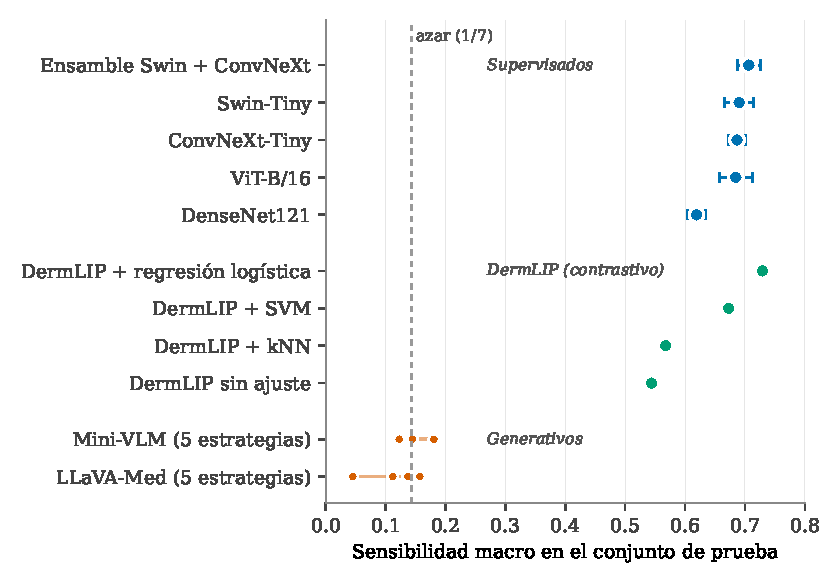
\includegraphics[width=0.85\textwidth]{Figures/Capitulos/04-Resultados-Clasificacion/resumen-sensibilidad-macro.pdf}
    \caption{Sensibilidad macro en la prueba de todos los clasificadores del capítulo. Los supervisados, con media y desvío de tres semillas; cada punto de los generativos es una estrategia.}
    \label{fig:res_resumen}
\end{figure}

Las pruebas de la Sección~\ref{sec:met_estadistica} confirman esa separación para los modelos sin ajuste, que entran
con la estrategia de generación en el caso de los generativos. En McNemar, los 15 pares de la familia de 21 que
comparan un supervisado con DermLIP, Mini-VLM o LLaVA-Med, o a estos tres entre sí, son significativos con la
corrección de Holm. La Tabla~\ref{tab:res_pruebas_vlm} muestra el tamaño de las diferencias en sensibilidad macro:
Swin-Tiny, ConvNeXt-Tiny y ViT-B/16 superan a DermLIP sin ajuste por entre 0.15 y 0.17, y a los generativos, por
alrededor de 0.5.

La única excepción es DenseNet121 frente a DermLIP. Su diferencia de sensibilidad macro no se distingue de cero, aunque
McNemar muestra que acierta más imágenes: DenseNet121 acierta 250 imágenes en las que DermLIP falla, frente a 85 en el
sentido contrario. Como en la comparación entre supervisados, la diferencia está en las clases mayoritarias, que pesan
mucho en el total de aciertos y poco en las métricas macro.

Entre los generativos, el intervalo de bootstrap de la sensibilidad macro de Mini-VLM incluye 1/7, de modo que
no se distingue del azar. El de LLaVA-Med queda apenas por encima, aunque su exactitud y su F1 macro siguen siendo
los de un modelo colapsado (Sección~\ref{sec:res_vlm}). Entre ellos, McNemar detecta que no aciertan las mismas
imágenes, pero la diferencia de sensibilidad macro no se distingue de cero, porque los dos aciertan pocas imágenes y
casi solo de la clase hacia la que colapsan.

\begin{table}[H]
    \centering
    \caption{Diferencia de sensibilidad macro entre cada supervisado y cada \gls{vlm} sin ajuste (semilla 42), con su IC del 95\,\%.}
    \label{tab:res_pruebas_vlm}
    \small
    \setlength{\tabcolsep}{4pt}
    \begin{tabularx}{\textwidth}{@{}>{\raggedright\arraybackslash}X ccc@{}}
        \toprule
        \textbf{Supervisado} & \textbf{DermLIP} & \textbf{Mini-VLM} & \textbf{LLaVA-Med} \\
        \midrule
        Swin-Tiny & 0.172 [0.116, 0.233] & 0.572 [0.522, 0.622] & 0.560 [0.510, 0.610] \\
        ConvNeXt-Tiny & 0.150 [0.092, 0.211] & 0.550 [0.501, 0.600] & 0.538 [0.488, 0.590] \\
        ViT-B/16 & 0.154 [0.105, 0.209] & 0.554 [0.503, 0.606] & 0.542 [0.490, 0.595] \\
        DenseNet121 & 0.050 [$-$0.016, 0.120] & 0.450 [0.398, 0.508] & 0.438 [0.385, 0.495] \\
        \bottomrule
    \end{tabularx}
\end{table}

La comparación deja abierta la posición de DermLIP con una cabeza entrenada, que se acerca a los supervisados en
sensibilidad macro pero no en F1 macro (Tabla~\ref{tab:res_dermlip}). Como esa cabeza se entrena sobre
\emph{HAM10000}, deja de ser un uso sin ajuste y no resuelve lo que motivaba usar un \gls{vlm}: obtener el diagnóstico
del modelo que genera el reporte.

\subsection{Costo computacional de los clasificadores}
\label{sec:res_costo_clasificadores}

Además del desempeño, la restricción de una GPU de consumo de la Sección~\ref{sec:met_tareas} exige que el
clasificador sea barato de ejecutar. La Tabla~\ref{tab:res_costo_clasificadores} reúne su costo en la RTX 4070 de la
Sección~\ref{sec:met_entorno}, con la misma precisión bf16 que la evaluación. Los cuatro modelos clasifican una
imagen en 20~ms o menos y ocupan menos de 0.7~GB de memoria de la GPU aun con lotes de 32 imágenes. Con esos lotes,
Swin-Tiny clasifica la prueba completa en poco más de un segundo, y con una imagen por vez, en unos 17 segundos.
Además, la cantidad de parámetros no ordena el tiempo de inferencia: DenseNet121, el modelo más chico, es el más lento
con una imagen por vez. Estos tiempos corresponden a una sola vista, y el \gls{tta} de la
Sección~\ref{sec:met_supervisados_receta} duplica las pasadas. Aun así, el costo de los clasificadores queda muy por
debajo de ese límite.

\begin{table}[H]
    \centering
    \caption{Costo de inferencia de los clasificadores en una RTX 4070 (bf16, una vista por imagen). La latencia se mide con una imagen por vez, y las imágenes por segundo, con lotes de 32.}
    \label{tab:res_costo_clasificadores}
    \small
    \setlength{\tabcolsep}{3pt}
    \begin{tabularx}{\textwidth}{@{}>{\raggedright\arraybackslash}X
        >{\centering\arraybackslash}p{1.9cm}>{\centering\arraybackslash}p{2.0cm}>{\centering\arraybackslash}p{2.0cm}
        >{\centering\arraybackslash}p{1.9cm}>{\centering\arraybackslash}p{2.0cm}@{}}
        \toprule
        & & \multicolumn{2}{c}{\textbf{Memoria máxima (GB)}} & & \\
        \cmidrule(lr){3-4}
        \textbf{Modelo} & \textbf{Parámetros (millones)} & \textbf{Una imagen} & \textbf{Lote de 32}
            & \textbf{Latencia (ms)} & \textbf{Imágenes por segundo} \\
        \midrule
        Swin-Tiny & 27.52 & 0.180 & 0.522 & 11.05 & 1\,353.3 \\
        ConvNeXt-Tiny & 27.83 & 0.179 & 0.407 & 4.99 & 1\,738.5 \\
        ViT-B/16 & 85.80 & 0.511 & 0.678 & 5.72 & 903.5 \\
        DenseNet121 & 6.96 & 0.052 & 0.216 & 19.89 & 1\,700.3 \\
        \bottomrule
    \end{tabularx}
\end{table}

Con el desempeño y el costo de las tres familias caracterizados, queda ubicar estos resultados frente a los de la
literatura.
